\chapter{Теоретические основы динамической симуляции огня}

В данной главе будут приведены основные теоретические сведения, которые
необходимы для введения в практическую часть диссертации. В главе будут
приведены необходимые определения из областей компьютерной графики и
математической симуляции, будут представлены рисунки и уравнения, поясняющие
информацию.

Глава состоит из двух разделов:
\begin{enumerate}
    \item Раздел ''Теоретические основы компьютерной графики'' предоставляет
        необходимые сведения об общих основах компьютерной графики.
    \item В разделе ''Динамическая симуляция огня'' можно найти описание\break{}
        структуры симуляции огня и ее элементов. В разделе приводятся формулы и
        алгоритмы, используемые в практической части.
\end{enumerate}.

\section{Теоретические основы компьютерной графики}

\subsection{Введение в компьютерную графику}

Для начала необходимо дать определение компьютерной или машинной графике.

\textbf{Компьютерная графика} --- это совокупность технических, математических и
программных средств и приемов, позволяющих осуществлять ввод и вывод из ЭВМ
графической информации без ручного преобразования информации в числовую или
графическую форму~\cite{SamalGraphics}.

Можно выделить три основных этапа формирования изображения электронной
вычислительной машиной:
\begin{itemize}
    \item построение модели объекта или сцены, содержащей несколько объектов
        (т\@.е\@. описание объектов и их связей в рамках евклидовой геометрии);
    \item подготовка модели к визуализации в зависимости от местонахождения
        наблюдателя (выполнение геометрических преобразований, удаление
        невидимых линий);
    \item визуализация с помощью заданного устройства отображения (отсечение по
        объему/окну видимости, формирование растрового представления, наложение
        текстуры, затенение, добавление дополнительных эффектов, вывод на
        терминал).
\end{itemize}

Изображение можно представить в виде множества точек, линий, строк текста и
закрашенных областей, называемых \textbf{примитивами}. При этом изображение чаще
всего описывается набором вершин, ребер и граней, формирующих в итоге множество
прямоугольников с заданными атрибутами и представляющих в совокупности один или
несколько объектов сцены. Следует отметить, что визуализация изображений, как
правило, выполняется на плоскости, т\@.е\@. итоговое изображение двухмерно, и,
таким образом, при отображении трехмерных объектов одним из обязательных шагов
является проективное преобразование.

Периферийные устройства вывода делятся по своему типу на растровые и векторные.
В настоящее время визуализация изображений производится в большинстве случаем
именно растровыми устройствами вывода. В растровых устройствах отображения точку
заменяет пиксель (от английского \textit{picture element}). \textbf{Пиксель} ---
это наименьшая часть изображения, с которой может работать алгоритм обработки
либо визуализации изображения.

Изображения, отображаемые на растровых устройствах, либо хранимые в виде
двухмерного массива значений пикселей --- растра, называются
\textbf{растровыми}. Процесс преобразования векторных моделей в растровые
изображения называется \textbf{растеризацией}.

\subsection{Библиотека OpenGL}

Практическая часть диссертации использует программный интерфейс \break{}для
создания трехмерной (3D) графики --- OpenGL\@. \textbf{OpenGL} --- это
программный интерфейс, который позволяет приложениям использовать и управлять
графической подсистемой устройства, на котором работает
OpenGL~\cite{OGLSuperbible}.

OpenGL может работать на различных устройствах от дорогостоящих профессиональных
рабочих станций до обычных настольных компьютеров, от игровых консолей до
мобильных телефонов. OpenGL предлагает стандартизированный интерфейс (API),
который предоставляет широкую портируемоесть и позволяет разработчикам
приложений фокусировать свое внимание на создании качественных продуктов,
разработке интересного контента, и увеличении производительности своих
приложений вместо того, чтобы беспокоиться о спецификациях платформы, для
которой они создают приложение.

OpenGL может разбивать поток работы на фундаментальные элементы и выполнять их
параллельно. Комбинации конвейеризации и параллелизма позволяет получить
максимальную производительность от современных графических процессоров.
Структура графического конвейера представлена на
рисунке~\ref{fig:graphicsPipeline}.
\begin{figure}[htb]
	\centering
	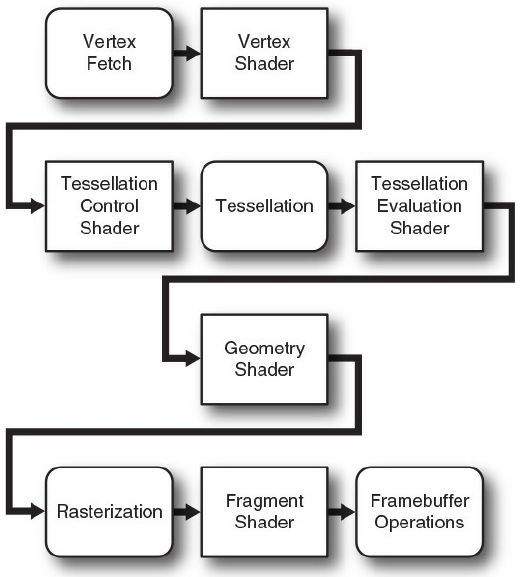
\includegraphics[width=0.75\textwidth]{graphicsPipeline}
	\caption{Упрощенная структура графического конвейера}%
    \label{fig:graphicsPipeline}
\end{figure}
На рисунке~\ref{fig:graphicsPipeline} блоки со скругленными краями представляют
собой фиксированные части, которые обычно реализованы как часть драйвера,
прошивки или другого системного ПО. Блоки с прямоугольными краями являются
программируемыми, это означает, что они могут выполнять шейдеры, предоставляемые
разработчиками ПО.

На момент написания диссертации существует 20 изданий спецификации
OpenGL~\cite{OpenGLHistory}. Номера версий и даты их публикации приведены в
таблице~\ref{table:OpenGLVersions}.
\begin{table}
\caption{Версии OpenGL}%
\label{table:OpenGLVersions}
\centering
\small
\begin{tabular}{| l | l |}
    \hline
    Версия & Дата публикации \\
    \hline
    OpenGL 1.0 & Январь 1992 \\
    OpenGL 1.1 & Январь 1997 \\
    OpenGL 1.2 & Март 1998 \\
    OpenGL 1.2.1 & Октябрь 1998 \\
    OpenGL 1.3 & Август 2001 \\
    OpenGL 1.4 & Июль 2002 \\
    OpenGL 1.5 & Июль 2003 \\
    OpenGL 2.0 & Сентябрь 2004 \\
    OpenGL 2.1 & Июль 2006 \\
    OpenGL 3.0 & Август 2008 \\
    OpenGL 3.1 & Март 2009 \\
    OpenGL 3.2 & Август 2009 \\
    OpenGL 3.3 & Март 2010 \\
    OpenGL 4.0 & Март 2010 \\
    OpenGL 4.1 & Июль 2010 \\
    OpenGL 4.2 & Август 2011 \\
    OpenGL 4.3 & Август 2012 \\
    OpenGL 4.4 & Июль 2013 \\
    OpenGL 4.5 & Август 2014 \\
    OpenGL 4.6 & Октябрь 2017 \\
    \hline
\end{tabular}
\end{table}
Старые версии OpenGL предлагали непосредственный режим работы (фиксированный
конвейер), который был простым способом для отрисовки графики.
Однако, большинство функционала было спрятана в библиотеке и у разработчиков не
было большого контроля над вычислениями. Начиная с версии 3.2 спецификации
началось стимулирование перехода разработчиков к новому API (core профиль),
который является версией спецификации, в которой убрана вся устаревшая
функциональность. Начиная с версии 3.3 радикальных изменений в спецификации не
происходило, в последующих версиях были добавлены некоторые функции для более
удобного выполнения частых задач. Разработанная в ходе диссертации система
использует спецификацию OpenGL версии 4.5, однако может быть легко портирована и
на более ранние версии.

Необходимо вернуться к обзору графического конфейера и дать определение понятию
''шейдер''. \textbf{Шейдеры} --- это небольшие программы, которые предназначены
для выполнения на графическом процессоре~\cite{LearnOGL}. Шейдеры могут
одновременно выполняться на тысячах вычислительный ядер ГП. Для вывода
изображения на экран необходимо наличие в шейдерной программе как минимум
вершинного и фрагментного шейдеров. Для написания шейдеров на OpenGL
используется \textbf{OpenGL Shading Language (GLSL)}. GLSL\@--- Си-подобный язык,
который также является частью спецификации OpenGL\@.

Одну из особенностей OpenGL является использование пяти различных координатных
систем:
\begin{itemize}
    \item локальное пространство (или пространство объекта);
    \item мировое пространство;
    \item пространство наблюдателя;
    \item пространство отсечения;
    \item экранное пространство.
\end{itemize}

Для преобразования координат из одного пространства в другое,
используется несколько различных матриц трансформации, среди которых, самыми важными
являются матрицы модели, вида и проекции. Координаты вершин появляются в
локальном пространстве как локальные координаты, и в дальнейшем преобразуются в
мировые координаты, потом в координаты вида, отсечения, и, наконец, все
все координаты приводятся к экранному пространству. На
рисунке~\ref{fig:spaceTransforms} представлена вся последовательность
преобразований и эффект, который оказывает каждое преобразование:
\begin{figure}[htb]
	\centering
	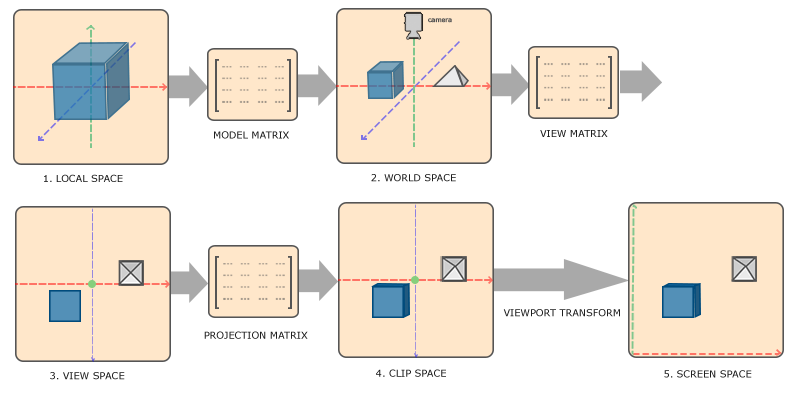
\includegraphics[width=\textwidth]{spaceTransforms}
	\caption{Преобразования систем координат в OpenGL}%
    \label{fig:spaceTransforms}
\end{figure}
\begin{enumerate}
    \item Локальные координаты это координаты объекта измеряемые относительно
        точки отсчета расположенной в центре объекта.

    \item На следующем шаге локальные координаты преобразуются в координаты
        мирового пространства, которое содержит все объекты сцены. Эти
        координаты измеряются относительно глобальной точки отсчета, единой для
        всех объектов расположенных в мировом пространстве.

    \item Далее происходит преобразование мировых координаты в координаты
        пространства наблюдателя таким образом, что каждая вершина становится
        видна как если бы на нее смотрели из камеры или из местоположения
        наблюдателя.

    \item После того, как координаты были преобразованы в пространство
        наблюдателя, необходимо спроецировать их в координаты пространства
        отсечения. Координаты пространства находятся в диапазоне от -1.0 до 1.0
        и определяют, какие вершины появятся на экране.

    \item И, наконец, происходит преобразование координат в экранное
        пространство. Размер пространства определяется размером окна, в котором
        происходит рендеринг изображения. В качестве точки отсчета берется
        нижний левый угол окна. Полученные координаты отсылаются растеризатору
        для превращения их во фрагменты (пиксели).
\end{enumerate}

Операцию приведения координат из пространства в модели в пространство отсечения
можно выполнить с помощью формулы (\ref{eq:mvp}).
\begin{equation}
  \label{eq:mvp}
  \text{V}_\text{clip} = \text{M}_\text{proj} \cdot \text{M}_\text{view} \cdot
  \text{M}_\text{model} \cdot \text{V}_\text{local}
\end{equation}
\begin{explanationx}
    \item [где] $\text{V}_\text{clip}$ --- координаты вершины в пространстве
        отсечения;
    \item $\text{M}_\text{proj}$ --- матрица преобразования в пространство
        отсечения;
    \item $\text{M}_\text{view}$ --- матрица преобразования в пространство
        наблюдателя;
    \item $\text{M}_\text{model}$ --- матрица преобразования в мировое
        пространство;
    \item $\text{V}_\text{local}$ --- координаты вершины в локальном
        пространстве.
\end{explanationx}

Матрицы не обладают свойством коммутативности, поэтому важно выполнять умножение
в правильном порядке. Умножение матриц следует читать в обратном порядке,
т\@.к\@. сначала к вершине применяется самая правая операция.

\section{Физика огня}

Перед тем, как приступить к симуляции огня, нужно глубже разобраться в природе
исследуемого объекта. Необходимо выделить разницу между огнем и пламенем,
дать определение процессу горения и описать его компоненты, сделать обзор
основных видов огня и глубже разобраться в физике процесса горения.

\subsection{Компоненты горения}

В русском языке нет четкого смыслового разделения слов пламя и
огонь\break{}\cite{WikiFlame}, однако в зарубежной литературе присутствует четкое
разделение понятий огонь (fire) и пламя (flame).

Несмотря на то, что стандарт СТ СЭВ 383--87~\cite{383-87} уже устарел, в нем
дается точное определение для ключевых терминов, используемых в диссертации. В
следующих подразделах также будут приведены определения из данного стандарта.

\textbf{Огонь} --- процесс горения, сопровождающийся пламенем или свечением.

\textbf{Пламя} --- зона горения в газовой фазе с видимым излучением.

Среди процессов химических веществ бывают случаи, когда вещество сгорает без
пламени~\cite{WikiFire}.

Обычно люди воспринимают горящий объект, словно горит сам объект. Однако, на
самом деле горит не сам объект, а топливо, которое он выделяет в окружающую
среду. Топливо подымается над поверхностью объекта из-за тепла, испаряется,
вступает в контакт к кислородом и воспламеняется. Таким образом, огонь нуждается
в совместном присутствии трех элементов: топливо, тепло и
кислород~\cite{USArmy}:
\begin{enumerate}
    \item \emph{Топливо}. Топливом может быть твердая, жидкая либо газообразная
        субстанция, также топливо должно химически разлагаться на газы или
        пар. Процесс разложения происходит под воздействием тепла.
    \item \emph{Тепло}. Тепло --- это мера молекулярной активности в объекте,
        увеличение температуры ведет к увеличению скорости движения молекул.
        Если к объекту приложено достаточно тепла, молекулы начинают двигаться
        настолько быстро, что могут покидать поверхность объекта. Так происходит
        процесс перехода топлива в газообразное состояние.
    \item \emph{Кислород}. Кислород является окисляющим агентом и поэтому
        необходим для процесса горения. На определенном уровне, частицы огня
        могут превращаться в частицы дыма из-за нехватки кислорода в воздухе,
        что вызывает неполное окисление.
\end{enumerate}

\section{Воспламенение объектов}

\textbf{Горение} --- экзотермическая реакция окисления вещества,
сопровождающаяся по крайней мере одним из трех факторов: пламенем, свечением,
выделением дыма~\cite{383-87}.

Процесс горения имеет следующие стадии:
\begin{enumerate}
    \item Окисление вызывает разложение горючего материала, происходит \break{}
        медленное выделение газов, включая водяной пар.  Процесс протекает
        непрерывно все время, в течение которого объект взаимодействует с
        окисляющим агентом, которым может выступать воздух.  При температуре
        окружающей среды окисление обычно происходит настолько медленно, что
        даже незаметно человеку. Горючие газы пока еще не могут воспламенятся на
        этой стадии.

    \item Скорость окисления возрастает с ростом температуры, в это время
        некоторые газы становятся воспламеняемыми. Точка, когда в воздухе
        находится достаточное количество пара, чтобы создать горючую смесь в
        воздухе, называется \emph{точкой вспышки}.

    \item В вышеупомянутой точке в выделенных газах присутствует слишком много
        углекислого газа и водяного пара, чтобы поддерживать пламя
        продолжительное время. Однако, тепло огня служит началом для вторичного
        процесса разложения, которое приводит к процессу устойчивого горения.
        Эта точка называется \emph{точкой воспламенения}, и она обычно находится
        на несколько градусов выше точки вспышки.

    \item Окисление может идти настолько быстро, что оно покрывает всю
        поверхность топлива и блокирует доступ к кислороду, препятствуя горению
        топлива и затрудняя проникновение тепла. Это задерживает распространение
        температуры возгорания вглубь горючего материала. Однако, с увеличением
        температуры топливо начинает светиться, воздух поступает внутрь для
        поддержания горения, и происходит горение топлива совместно с
        выделяемыми газами.

    \item Если тепла выделяется больше, чем теряется из-за проводимости,
        конвекции или излучения, огонь будет поддерживаться и появится пламя.
        Горение будет поддерживаться, пока либо тепло, горючее, или окисляющий
        агент не будут убраны из системы.
\end{enumerate}

\subsection{Классификация огня}

Следуя классификации, предложенной в~\cite{nielsen}, огонь может быть разделен
по визуальным характеристикам на следующие группы:
\begin{enumerate}
    \item \emph{Спокойный огонь}. Типичным примером спокойного огня
        является \break{} огонь свечи. Спокойный огонь редко нарушается
        воздействием внутренних либо внешних сил. Таким образом, огонь остается
        спокойным и практически не движется, если движется вообще.

    \item \emph{Свободно питаемый огонь}. Свободно питаемый огонь не
        испытывает нехватки топлива и получает достаточное количество кислорода,
        также количество топлива и кислорода варьируется в зависимости от
        времени и местоположения. Это существенно отличается он спокойного огня,
        который имеет более или менее постоянное и контролируемое количество
        топлива и доступного кислорода на протяжении всего времени горения и во
        всех областях огня.

    \item \emph{Сильный огонь}. В сильном огне, внешние силы оказывают сильное
        влияние на огонь, вызывая неравномерную подпитку огня и распространение
        топливных компонентов в направлениях, отличных от вертикального. Пожары
        крайне переменчивы и крайне непредсказуемы из-за сложности лежащих в их
        основе систем и большого количества влияющих сил.

    \item \emph{Огонь, подаваемый под давлением}. Огонь, подаваемый под
        давлением --- это свободный огонь, вектора скорости которого направлены
        в сторону, в которую происходит выброс топлива в воздух.

    \item \emph{Детонации и взрывы}. \emph{Взрыв} — это процесс, в котором за
        короткое время в ограниченном объёме выделяется большое количество
        энергии и образуются газообразные продукты взрыва, способные совершить
        значительную механическую работу или вызвать разрушения в месте
        взрыва~\cite{WikiDetonation}. В \emph{детонациях} используется изначально
        сжатое топливо; возгорание вызывает взрывную волну, которая вызывает
        серию небольших взрывов, которые создают новые взрывные волны.
\end{enumerate}

Также хочется отметить такой процесс, как пожар. \textbf{Пожар} ---
неконтролируемое горение, приводящее к ущербу. При моделировании пожаров
основной упор делается на расчет скорости распространения дыма и огня, вместо
реалистичной визуализации зачастую используется схематичная. Моделирование
пожаром находится за пределами данного исследования.

\subsection{Визуальное восприятие огня}%
\label{section:firePerception}

Огонь является довольно сложным природным феноменом. В данном подразделе будет
приведен обзор основных физических особенностей, влияющих на визуальное
восприятие человеком огня. В данном разделе будут приведены моменты касательно
спектра огня, сопротивления воздуха, вызывающего эффект подергивания,
формирование и вид сажи и дыма.

Обычно в естественных науках огонь рассматривают в качестве излучателя черного
тела, для описания цвета. Черное тело испускает фотоны различных цветов, от
черного до белого, проходя через красный, оранжевый и желтый. Цветовой спектр
излучения черного тела приведен на рисунке~\ref{fig:fireSpectrum}. Данный спектр
несколько ограниченно описывает световое излучение, испускаемое в процессе
горения, поскольку он не учитывает вклад различных примесей, которые могут
сильно влиять на цвет пламени.
\begin{figure}[htb]
	\centering
    
\includegraphics[width=0.75\textwidth]{fireSpectrum}
	\caption{Спектр излучения черного тела}%
    \label{fig:fireSpectrum}
\end{figure}

Взаимодействие цвета и температуры можно рассмотреть на примере горения свечи,
представленной на рисунке~\ref{fig:candle}.
\begin{figure}[htb]
	\centering
    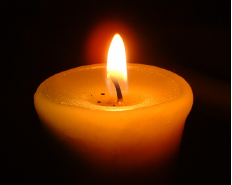
\includegraphics[width=0.4\textwidth]{candle}
	\caption{Горение свечи}%
    \label{fig:candle}
\end{figure}
Часть пламени, наиболее близкая к фитилю, невидима, изменяясь постепенно к
голубоватому цвету на границе и у основания пламени. В самой горячей точке пламя
приобретает белый цвет. Остальные регионы пламени имеют светло-желтый цвет,
который постепенно переходит в оранжевый или красный у вершины. Быстрое
сравнение цветов пламени свечи и цветовой палитры излучения черного тела
показывает ограничения палитры, поскольку она не нацелена на отображение пламени
на восковом топливе.

Необходимо также описать факторы, влияющие на движение огня. Следующий пример,
иллюстрирующий движение горячего турбулентного газа был взят
из~\cite{Foster1997ModelingTM}. Представим старомодный паровой двигатель,
выпускающий\break{}струю горячего пара из своего бойлера. В самом начале,
ведущим фактором, влияющим на движение газа, является скорость, с которой его
выпустили в окружающую среду. В то время, как пар смешивается с более медленно
двигающимся воздухом, пар испытывает \emph{сопротивление воздуха} (drag), и
начинает вращаться в некоторых местах. Это вращение усиливает смешивание с
воздухом и вызывает появление завихрений, которые мы можем наблюдать при
смешивании газов.  Согласно~\cite{Foster1997ModelingTM}, следующим важным
фактором, влияющим на движение газа является температура. Как только струя пара
была выпущена, она поднимается вверх, и более горячие участки подымаются
быстрее, чем области, которые смешались с более холодным воздухом. В то время,
как газ подымается, он испытывает внутреннее сопротивление воздуха, которое
создает еще больше турбулентного вращения. Этот эффект известен под названием
\emph{термальной плавучести} (thermal buoyancy). Влияние сопротивления воздуха и
термальной плавучести на движение газов приведено на
рисунке~\ref{fig:gasMotion}.
\begin{figure}[htb]
	\centering
    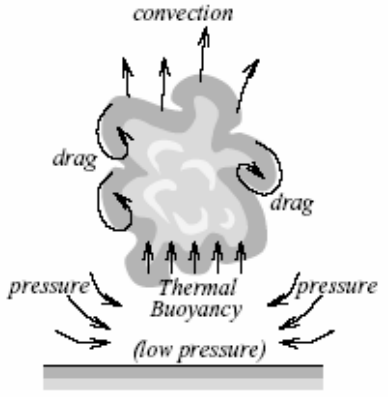
\includegraphics[width=0.4\textwidth]{gasMotion}
	\caption{Движение горячего газа}%
    \label{fig:gasMotion}
\end{figure}

Наконец, дым и сажа появляются при недостатке в ядре огня кислорода для
поддержания процесса горения. На выходе получается неполное сгорание, которое
производит такие побочные продукты как сажа. Дым является результатом смешивания
сажи с водой, что обычно происходит в процессе горения. Дым от огня зачастую
очень темный из-за высокого содержания углекислого газа в воздухе. Однако, из-за
влияния различных компонентов горючего материала или других побочных продуктов
горения, в воздух могут подыматься примеси и других цветов. Например, пар имеет
серый цвет (количество воды преобладает над количеством сажи).

\section{Особенности рендеринга в реальном времени}

В~\cite{Young1982RealTL} приводится определение системы реального времени
''любой активности по обработке системы либо системы, которой необходимо
отвечать на внешние входные данные за конечный и определенный период.'' Таким
образом, симуляция огня в режиме реального времени --- это симуляция, поведение
и окружение которой должно быть рассчитано за период времени, соизмеримый с ее
поведением и окружением в реальном мире. Это отличается от конвейера,
используемого в оффлайн симуляции при производстве фильмов, где расчет каждого
кадра может занимать минуты либо часы.

В общем случае, в компьютерной графике существует большой отрыв между скоростью
и реализмом. В приложениях реального времени наибольший приоритет отдается
скорости. Таким образом, ключевой проблемой симуляции в реальном времени
является поиск баланса между количеством вычислений для достижения оптимального
результата, не допуская при этом падения частоты кадров ниже минимальной
допустимой границы.

Для каждого желаемого атрибута необходимо выбрать оптимальный алгоритм для
конкретного случая. Такая оптимальность зачастую достигается внедрением
разнообразных ухищрений, которые имеют слабую связь с поведением объектов в
реальном мире, однако они позволяют достичь желаемого эффекта. Некоторые примеры
таких ухищрений будут описаны ниже в этом разделе. Суть идеи в том, что пока
симуляция показывает визуально приемлемые результаты и выполняется с достаточно
быстрой скоростью, скорее всего никто не заметит особых различий. Использование
таких ухищрений не является чем-то зазорным, поскольку они с самого присутствуют
в индустрии компьютерной графики с самого момента ее появления. По факту, на
момент своего появления вся индустрия компьютерной графики сплошь состояла из
таких ухищрений.

В общем случае задача симуляции огня может быть разбита на три
непересекающихся подзадачи~\cite{Perry94synthesizingflames}:
\begin{itemize}
	\item моделирование;
	\item анимация;
	\item визуализация.
\end{itemize}

В первую очередь необходимо выбрать подходящую внутреннюю структуру, или модель,
для симуляции. Далее, требуется выбрать способ анимации --- метод, с помощью
которого будет происходить взаимодействие с моделью. Техника анимации служит для
того, чтобы оживить модель, привести ее в движение. Наконец, модель и ее
анимацию необходимо отрисовать на экране, используя для этого некоторые
примитивы визуализации (полигоны, текстуры, сферы, воксели и т.п.).

Альтернативная схема была предложена в~\cite{realistic_sim}, в которой авторы
делают акцент на алгоритмах распространения огня. Фаза моделирования в данном
случае является одним из этапов при разработке алгоритмов распространения
пламени. Схема, предложенная в данной работе, представлена на
рисунке~\ref{fig:simStages}.

\begin{figure}[htb]
	\centering
    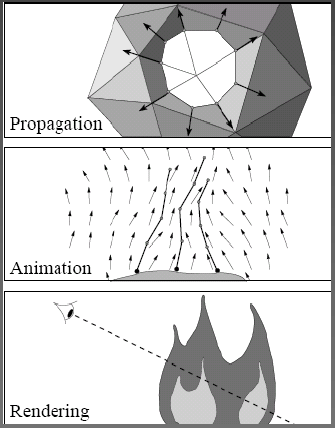
\includegraphics[width=0.4\textwidth]{simStages}
    \caption{Структура симуляции, предложенная в~\cite{realistic_sim}}%
    \label{fig:simStages}
\end{figure}

Более подробный обзор каждой стадии симуляции будет основан на схеме,
предложенной в~\cite{realistic_sim}. В последующих подразделах будут
последовательно рассмотрены каждая из стадий симуляции, и будут описаны нюансы
их взаимодействия.

\subsection{Моделирование и визуализация огня}

Стохастические методы моделирования огня, такие как поля турбулентности и шумов
очень эффективны при создании реалистичного огня в 2D графике, но являются
крайне неэффективными по количеству операций для использования в 3D анимациях в
реальном времени, независимо от выбранной техники визуализации. Альтернативой
может быть эффективно реализованная объемная модель рендеринга, использующая
воксели в качестве примитива визуализации, помогает достичь приемлемую для
интерактивных приложений частоту кадров. Однако, при использовании данной модели
сложно добиться реалистичных результатов, поскольку поверхность огня не имеет
четких границ. Наиболее быстрым методом является объемное моделирование с
использованием полигонов для визуализации; отрисовка полигонов происходит крайне
быстро, однако полигоны не лучшее средство для визуализации языков пламени,
вихрящегося дыма и частиц сажи, и поэтому обычно полигоны пораждают довольно
грубые и низкокачественные результаты. Где-то между ними находится моделирование
с помощью систем частиц, данный метод может работать с желаемой скоростью, в
зависимости от выбранного масштаба, который выбирается из расчета необходимого
уровня детализации и выбранных техник анимации и визуализации. Как было описано
в обзоре литературы, большинство симуляций огня используют системы частиц того
или иного вида. Этот метод также используется в практической части. Поэтому
дальнейшее описание симуляции будет сфокусировано на применении систем частиц.
Системы частиц позволяют моделировать трехмерное поведение огня в интуитивной и
простой манере, однако, они имею и свой набор недостатков, которые будут описаны
ниже.

Одной из проблем, связанных с системами частиц, является то, что они
предполагают одно и то же окружение для всех частиц в системе. Решением этой
проблемы является разбиение окружения на более мелкие части, называемые
\emph{полями}~\cite{nielsen}. Поле содержит информацию, касательно определенного
участка сцены, который зачастую представляет форму куба или прямоугольной
призмы, либо любой другой формы, которая может быть использована для создания
мозаики, описывающей окружение. Однако, поля оказывают большую нагрузку на
оперативную память. В идеальном случае, решетка должна охватывать всю сцену,
которая может быть подвержена влиянию огня, при этом ячейки должны иметь
достаточно малый размер, чтобы оказывать достаточно точное влияние на симуляцию.
Это является крайне сложной задачей для поиска оптимального решения, т\@.к\@.
установка всего лишь $10$ кубов в одном из измерений кубической сцены приводит к
$10^3 = 1000$ полей в сцене, при этом каждый кадр необходимо производить расчет
каждого поля. При этом, данная цифра является довольно заниженной оценкой,
поскольку окружение симуляции огня в основном имеет форму отличную от
кубической, и поэтому высота зачастую значительно превышает размеры ширины либо
глубины.

Второй проблемой систем частиц является то, что они требуют наличие огромного
количества частиц для полной симуляции системы, т\@.к\@. в идеальном случае
необходимо заниматься моделированием взаимодействий на молекулярном уровне.
Понятно, что задачу необходимо обобщить. \emph{Текстурный маппинг} является
одной из форм такого обобщения, и некоторые варианты данного метода является
часто используемым способом для достижения частоты кадров, необходимой при
симуляции в режиме реального времени. Пример текстурных карт представлен на
рисунке~\ref{fig:fireSplats}.
\begin{figure}[htb]
	\centering
    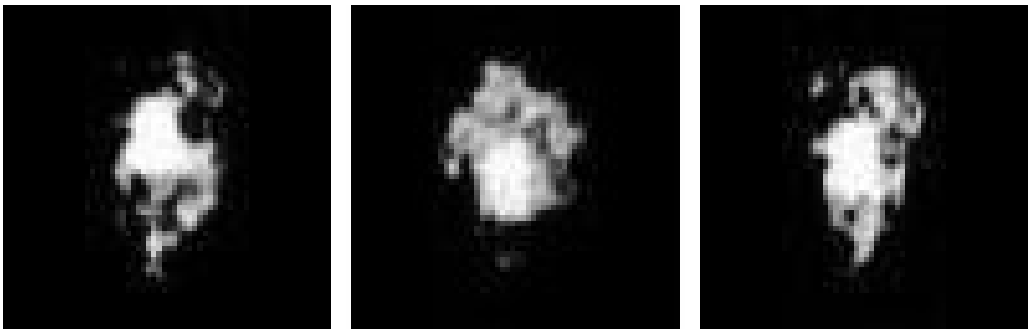
\includegraphics[width=0.5\textwidth]{fireSplats}
    \caption{Текстурные сплэты, созданные на основе
    фотографий~\cite{FireSplats}}%
    \label{fig:fireSplats}
\end{figure}
В методе текстурного маппинга статическая анимация огня накладывается на
полигоны, которые находятся на месте частиц в системе. Суть такого маппинга в
том, что теперь одна частица отображает целый кластер частиц, расположенных, как
на текстуре. Полигон обычно направлен на зрителя, когда тот перемещается по
сцене, с помощью вращения вдоль оси $y$. Однако, как можно заметить, в таком
случае полигон может быть направлен на зрителя только тогда, когда зритель
передвигается вдоль осей $x$ и $y$, и, как можно предположить, огонь будет
выглядеть довольно странно, если смотреть на него сверху, особенно сильно это
будет заметно, если посмотреть на сцену под острым углом. Еще одной проблемой,
связанная с использованием текстурного маппинга, является то, что освещение
сцены будет считать полигоны плоской поверхностью, и применять соответствующие
эффекты освещения к огню, которые, конечно, будут выглядеть крайне
нереалистично.

Одним из улучшений текстурного маппинга является текстурный сплэттинг, который
является техникой для симуляции объемного рендеринга. В текстурном сплэттинге
битовая карта складывается с картой прозрачности, таким образом битовая карта
становится частично прозрачной. Другими словами, текстурные приближения на
разных уровнях накладываются друг на друга с использованием смешивания.

Другим улучшением текстурного маппинга является использование
последовательностей изображений реального огня, вместо постоянного
переиспользования одной и той же текстуры для каждого полигона. Данное улучшение
помогает улучшить визуальное восприятие сцены с помощью уменьшения количества
статических элементов. Эта техника хорошо себя зарекомендовала и позволяет
получать довольно убедительные результаты.

Как можно заметить, метод текстурного маппинга позволяет успешно встраивать
заранее отрисованные элементы в симуляции в режиме реального времени. Так же
можно заметить, что при встраивании 2D текстур в 3D симуляцию, симуляцию уже
сложно назвать по-настоящему трехмерной. Однако, это является одним из тех
ухищрений, про которые шла речь в начале этого раздела. У текстур нет аналога в
реальном мире, поэтому это является своеобразным ухищрением. Текстуры слегка
смывают различие между 2D и 3D симуляцией, однако, использование текстур 2D
текстур в трехмерной симуляции довольно популярно, поскольку позволяет
существенно снизить вычислительную нагрузку. Разработанная в ходе исследования
система также использует данный прием.

\subsection{Анимация огня}

Существует множество способов анимации огня. Среди них можно выделить подходы,
использующие дифференциальные уравнения. Данные подходы позволяют получить
точные анимации, однако, они требуют отслеживания огромного числа переменных.
Производимые с помощью данных подходов симуляции тяжело контролировать,
поскольку их параметрами являются физические константы, чью взаимосвязь с
желаемыми визуальными характеристиками зачастую крайне сложно установить.
Вдобавок значения для этих параметров необходимо подбирать вручную, поскольку
природа огня еще до конца не изучена. Наиболее важно то, что эти подходы требуют
выполнения значительного количества вычислений, и поэтому их сложно применять в
симуляции в режиме реального времени.

Решением данной проблемы может быть попытка реализовать лишь наиболее важные
физические свойства огня, которые описаны в
разделе~\ref{section:firePerception}. Далее необходимо добиваться максимально
возможной реалистичности и\break{}эффектности каждого из компонентов. При этом следует
уделить внимание тому, чтобы реализация выглядела достаточно правдоподобно и не
была слишком уж заточена под конкретную сцену. Необходимо стремиться к более
элегантным решениям.
